% Glucose System Block Diagram
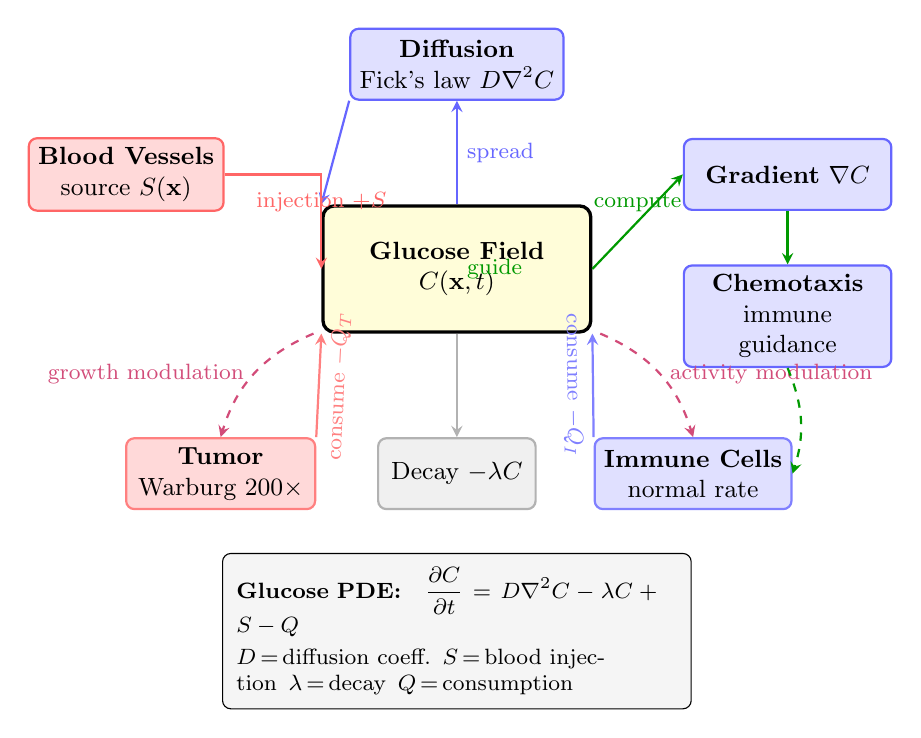
\begin{tikzpicture}[
  block/.style={draw, rounded corners=3pt, minimum width=2.4cm, minimum height=0.9cm,
                align=center, font=\small, thick},
  field/.style={draw, rounded corners=4pt, minimum width=3.4cm, minimum height=1.6cm,
                align=center, font=\small, thick, fill=yellow!15, line width=1.2pt},
  src/.style={block, fill=red!15, draw=red!60},
  proc/.style={block, fill=blue!12, draw=blue!60},
  cons/.style={block, fill=orange!15, draw=orange!60},
  arrow/.style={->, >=stealth, thick},
  dasharrow/.style={->, >=stealth, thick, dashed, purple!70},
]

% Central field
\node[field] (F) at (0, 0) {\textbf{Glucose Field}\\$C(\mathbf{x},t)$};

% Top: Diffusion
\node[proc] (diff) at (0, 2.6) {\textbf{Diffusion}\\Fick's law $D\nabla^2 C$};
\draw[arrow, blue!60] (F.north) -- (diff.south) node[midway, right, font=\footnotesize] {spread};
\draw[arrow, blue!60] (diff.south west) -- (F.north west);

% Left: Blood Vessels source
\node[src] (bv) at (-4.2, 1.2) {\textbf{Blood Vessels}\\source $S(\mathbf{x})$};
\draw[arrow, red!60] (bv.east) -- (F.west |- bv) -- (F.west)
  node[midway, above, font=\footnotesize] {injection $+S$};

% Right: Gradient & Chemotaxis
\node[proc, text width=2.4cm] (grad) at (4.2, 1.2) {\textbf{Gradient} $\nabla C$};
\node[proc, text width=2.4cm] (chem) at (4.2, -0.6) {\textbf{Chemotaxis}\\immune guidance};
\draw[arrow, green!60!black] (F.east) -- (grad.west) node[midway, above, font=\footnotesize] {compute};
\draw[arrow, green!60!black] (grad) -- (chem);

% Bottom-left: Tumor consumer
\node[cons, fill=red!15, draw=red!50] (tum) at (-3.0, -2.6) {\textbf{Tumor}\\Warburg 200$\times$};
\draw[arrow, red!50] (tum.north east) -- (F.south west)
  node[midway, below, sloped, font=\footnotesize] {consume $-Q_T$};

% Bottom-right: Immune consumer
\node[cons, fill=blue!12, draw=blue!50] (imm) at (3.0, -2.6) {\textbf{Immune Cells}\\normal rate};
\draw[arrow, blue!50] (imm.north west) -- (F.south east)
  node[midway, below, sloped, font=\footnotesize] {consume $-Q_I$};

% Below center: Decay
\node[proc, fill=gray!12, draw=gray!60, minimum width=2.0cm] (dec) at (0, -2.6) {Decay $-\lambda C$};
\draw[arrow, gray!60] (F.south) -- (dec.north);

% Dashed feedback arrows
\draw[dasharrow] (F.south west) ++(-0.1, 0) to[bend right=25]
  node[midway, left, font=\footnotesize, text=purple!70] {growth modulation} (tum.north);
\draw[dasharrow] (F.south east) ++(0.1, 0) to[bend left=25]
  node[midway, right, font=\footnotesize, text=purple!70] {activity modulation} (imm.north);

% Chemotaxis feedback
\draw[arrow, green!60!black, dashed] (chem.south) to[bend left=20] (imm.east)
  node[midway, right, font=\footnotesize] {guide};

% PDE equation box
\node[draw, rounded corners=3pt, fill=gray!8, inner sep=5pt, font=\footnotesize,
      text width=5.6cm, align=left] (pde) at (0, -4.6) {%
\textbf{Glucose PDE:}\quad
$\displaystyle\frac{\partial C}{\partial t} = D\nabla^2 C - \lambda C + S - Q$\\[2pt]
$D$\,=\,diffusion coeff.\enspace
$S$\,=\,blood injection\enspace
$\lambda$\,=\,decay\enspace
$Q$\,=\,consumption};

\end{tikzpicture}
